\chapter{Design} \label{cha:design}

With the prior analysis completed, the design decisions for the robot can be made. This chapter will contain a description of all the design decisions the implementation of the \projname{} will be based on. A platform has already been chosen, but there is also the matter of choosing the optimal operating system. The chosen operating system and the reasons for why it was chosen will be explained. Afterwards the functionality of the robot will be described, as well as the chosen algorithm for solving the problem, described in \secref{sec:problem-description}. This will result in the final requirements for the \projname{}-prototype.

% Language
\section{Operating system and programming language} \label{sec:os_and_proglanguage}
Since the LEGO Mindstorm NXT was chosen as the platform for the prototype robot, it puts some limitations on the choice of OS and programming language. It is required to use an OS that is supported by the NXT Intelligent Brick and the programming language must furthermore be supported by the chosen OS.

A few different OSes were considered for the \projname{}. The default NXT firmware IDE allows for simple drag-and-drop programming in the accompanying LEGO NXT-G software, for creating simple sample robots quickly. Another IDE called BricxCC, also used with the default firmware, uses the programming language Not eXactly C (NXC) and Next Byte Codes (NBC). The default firmware allows for programming both simple and more advanced robots. 

A considered custom firmware was leJOS NXJ, that uses the programming language Java. The leJOS NXJ OS contains a tiny Java virtual machine to execute the code \citep{lejos}. This implies that, had this OS been chosen, the source code would be written in Java.

Another of the considered custom firmwares is nxtOSEK. nxtOSEK is a hybrid between the device drivers of leJOS NXJ, the TOPPERS/ATK Kernel, and the TOPPERS/JSP Real-Time OS. It supports programming in ANSI C/C++ using GCC (GNU ARM) and contains a C and C++ API for the NXT sensors and motors~\citep{nxtosek, toppers_atk, toppers_jsp, nxtOSEK2, nxtosek_api}.

nxtOSEK supports multithreading and real-time multi tasking features, and more importantly for the \projname{}, events are also supported. Bluetooth connection is supported, both brick to brick, and brick to pc, where R/C and Data Logging possibilities exist.

The default OS is more restrictive than some of the alternatives. Because of this, it was decided use one of the custom firmwares. The C/C++ languages were favoured over Java and were the main reason why nxtOSEK was chosen over leJOS.







%Since the LEGO Mindstorm NXT was chosen as the platform for the prototype robot, it puts some limitations on the choice of OS and programming language. It is required to use an OS that is supported by the NXT Intelligent Brick and the programming language must furthermore be supported by the chosen OS.

%A few different OSes were considered for the \projname{}. The default NXT firmware IDE allows for simple drag-and-drop programming in the accompanying LEGO NXT-G software, for creating simple sample robots quickly. Another IDE called BricxCC, also used with the default firmware, uses the programming language Not eXactly C (NXC) and Next Byte Codes (NBC). NXC is a high-level open-source language similar to the C language, build on the NBC compiler. 

%The default firmware and the supported programming languages and tools associated, allows for programming both simple and more advanced robots. However it is still more restrictive than some of the alternatives. Because of this, it was decided to look at a couple of custom firmwares.  

%One of the considered custom firmwares was leJOS NXJ, that uses the programming language Java. The leJOS NXJ OS contains a tiny Java virtual machine to execute the code \citep{lejos}. It also includes all classes in the NXJ API \citep{nxj} as well as all the tools needed to upload programs to the NXT brick. This implies that, had this OS been chosen, the source code of this project would be written in Java and then apply Java methods to invoke the API.

%Another of the considered firmwares is nxtOSEK. nxtOSEK is a hybrid between the device drivers of leJOS NXJ, the TOPPERS/ATK Kernel, and the TOPPERS/JSP Real-Time OS, along with further code to make these work together. It supports programming in ANSI C/C++ using GCC (GNU ARM) and contains a C and C++ API for the NXT sensors and motors. The C and C++ API calls are available through ECRobot, that extends the C++ language with the necessary commands to manipulate the LEGO NXT hardware~\citep{nxtosek, toppers_atk, toppers_jsp, nxtOSEK2, nxtosek_api}.

%nxtOSEK includes a variety of useful features. Like leJOS it contains all the tools needed to upload programs to the NXT brick. It is possible to use the Eclipse CDT IDE to write and compile programs and upload them to the NXT brick. It supports multithreading and real-time multi tasking features provided by TOPPERS, and more importantly for the \projname{}, events are also supported. It supports Bluetooth connections, both from the brick to PC and from NXT Brick to NXT Brick. Furthermore, connecting a brick to the PC through Bluetooth, R/C and Data Logging features is provided by the NXT Gamepad.

%The C/C++ languages were favoured over Java and were the main reason why nxtOSEK was chosen over leJOS.

%BricxCC \citep{bricxcc} is an Integrated Development Environment (IDE) for programming LEGO NXT robots on the default firmware. BricxCC includes support for programming the LEGO Mindstorms NXT brick using the programming languages Not eXactly C (NXC) and Next Byte Codes (NBC). NBC is a simple open-source language with an assembly language syntax, and NXC is a high-level open-source language similar to C, built on the NBC compiler.



%The default firmware and the supported programming languages and tools associated, allows for programming both simple and more advanced robots. However it is still more restrictive than some of the alternatives. Because of this, it was decided to look at a couple of custom firmwares. One of the considered custom firmwares was leJOS. The leJOS NXJ \citep{lejos} OS contains a tiny Java virtual machine to execute the users code. It also includes all classes in the NXJ API \citep{nxj} as well as all the tools needed to upload programs to the NXT brick. It supports programming in an object-oriented language, Java. This implies that, had this OS been chosen, the source code of this project would be written in Java or a similar language that can be compiled to Java bytecode and then apply Java methods to invoke the API.

%The last of the considered OSes, which also was the one chosen for this project, was nxtOSEK. nxtOSEK \citep{nxtosek} is a hybrid between the device drivers of leJOS NXJ, the TOPPERS/ATK \citep{toppers_atk} Kernel, and the TOPPERS/JSP \citep{toppers_jsp} Real-Time OS, along with further code to make these work together. It supports programming in ANSI C/C++ using GCC (GNU ARM) and contains a C and C++ API for the NXT sensors and motors. The C and C++ API calls are available through ECRobot, described in \secref{subsec:ecrobot}. These languages were favoured over Java and were the main reason why nxtOSEK was chosen over leJOS.

%nxtOSEK includes a variety of useful features. Like leJOS it contains all the tools needed to upload programs to the NXT brick. It is possible to use the Eclipse CDT IDE to write and compile programs and upload them to the NXT brick. It supports multithreading and real-time multi tasking features provided by TOPPERS, and more importantly for the \projname{}, events are also supported. It supports Bluetooth connections, both from the brick to PC and from brick to brick (one NXT to another NXT). This means that two NXT bricks can communicate with each other and be used in a master-slave relationship. Furthermore, connecting a brick to the PC through Bluetooth, R/C and Data Logging features is provided by the NXT Gamepad.

%\subsection{ECRobot} \label{subsec:ecrobot}
%Along with the nxtOSEK firmware comes the ECRobot API. This extends the C++ language with the necessary commands to manipulate the LEGO NXT hardware. The ECRobot C API was originally developed for a MATLAB Model-Based Design environment for the first LEGO Mindstorm NXT release. With the release of LEGO NXT 2.0 a ECRobot C++ API was developed. The update from C to C++ took the ECRobot from a structured imperative API to an object oriented API, which allowed the different motors and sensors to be sorted into device classes~\citep{nxtosek_api}.



%control the motors and different input sensors.

% Functionality description
\section{Functionality description} \label{sec:functionality_description}
In this section the overall functions and the different parts of the \projname{} are described. The fully built \projname{} includes four sensors and four servo motors, which means that it also includes two NXT Bricks, as it only supports three outputs pr. Brick for the motors. The robot drives in the environment, using the interactive servo motor until it locates an object, using the ultrasonic sensor, or the black boundary using the colour sensor. If it locates an object, the master brick transmit a signal to the slave brick to commence the arm task. During this time, the robot stands still, waiting on a signal. All the components and how they are connected to the NXT Bricks is shown in \figref{fig:robot_overview}. 

\subsection{Brick communication}
The two LEGO NXT bricks used for the robot is required to communicate in order to start and stop certain tasks. The integrated Bluetooth 2.0 module is used for communication between the NXT Bricks. One of the two LEGO NXT Bricks is chosen to be the master and the other one is the slave. The master unit controls the primary task of the robot, while the slave is used to handle a smaller, parallel task when receiving instructions from the master unit.

\subsection{Colour sensor} 
The robot is equipped with two colour sensors on the front of the robot, at each side. This is used to detect the black lines that specify the boundary of the environment. Based on the returned light the colour sensors return the RGB value to the LEGO NXT brick. The two colour sensors are handled by the master unit. 

\subsection{Ultrasonic sensor}
The ultrasonic sensor is placed in the front of the robot, just under the claw. This is used to detect the distance to the objects in front of the robot. The master unit is controlling the ultrasonic sensor.
%The ultrasonic sensor can measure the distance from the sensor to other objects. The robot use the ultrasonic sensor for detecting the distance to other object in front of the robot. The ultrasonic sensor are also controlled by the master unit. 

\subsection{Compass sensor}
The compass sensor is placed on the top or the robot, at the end of an arm, so that it is located as far from the bricks and motors as possible. This is to reduce the noise from the bricks and motors magnetics fields. The sensor is pointing in the same direction as the robot.

The compass sensor is used to help ensure precision in the robots movement. This increased precision in movement is used when searching for objects, and when turning to the exact degree where the next object is located. When the object are discovered during the scanning phase, their location are mapped according to distance and the angle between them.

\subsection{Interactive servo motor}
The four interactive servo motors is used for two tasks. The first task is to move the robot around the environment. This includes driving forward, backward, and turning. The second task is the arm and the claw. This task consist of squeezing the claw around a detected object and holding this until the arm has reached the point, where the claw can let go of the object, and this lands in the storage behind the robot. Then the arm returns to the starting position, ready to grab a hold of new objects. Both task use 2 motors. The driving task is handled by the master unit, and the arm task is handled by the slave unit.

\subsection{Motor controller}
The tests in \secref{sec:servo_motor} proves that the motors used in the project are not very precise. It was decided to implement a motor controller to solve the precision issues. The objective for the motor controller is to ensure that the motors reach the same distance at the same time. 

The controller takes as input how many steps each motor has turned at any given time. Based on the steps, and the direction, the speed is increased or decreased on the left motor. The left motor is selected as the motor where the speed is changed, and the right motor moves at constant speed. The motor controller also ensures that the robot stops at the targeted number of steps $+/-$ an acceptable error margin.

It is not possible to make the motors 100\% precise because of the minimum speed for driving the robot is too high. This is due to the construction of the robot. To deal with this problem, a reasonable error margin is chosen. The error margin is used in two cases: First if the motors difference in steps is inside this error margin the robots speed is not adjusted. Secondly if the motor is inside the target steps, the robot will stop moving.  

The result of the controller is a robot that, even though the hardware is imprecise, moves straight and behave as expected.


$motorR\_ahead \leftarrow Motor~L~steps~<~Motor~R~steps$
$motorL\_ahead \leftarrow Motor~L~steps~>~Motor~R~steps$



$moving\_forward$

$ motor\_power\_increased \leftarrow moving\_forward \land motorR\_ahead \land \lnot motorL\_ahead$


$motor_power_decreased \leftarrow $ 

\fxnote{Se link i kommentar under fxnote}
% http://artint.info/html/ArtInt_106.html

\begin{figure}[H]
     \center{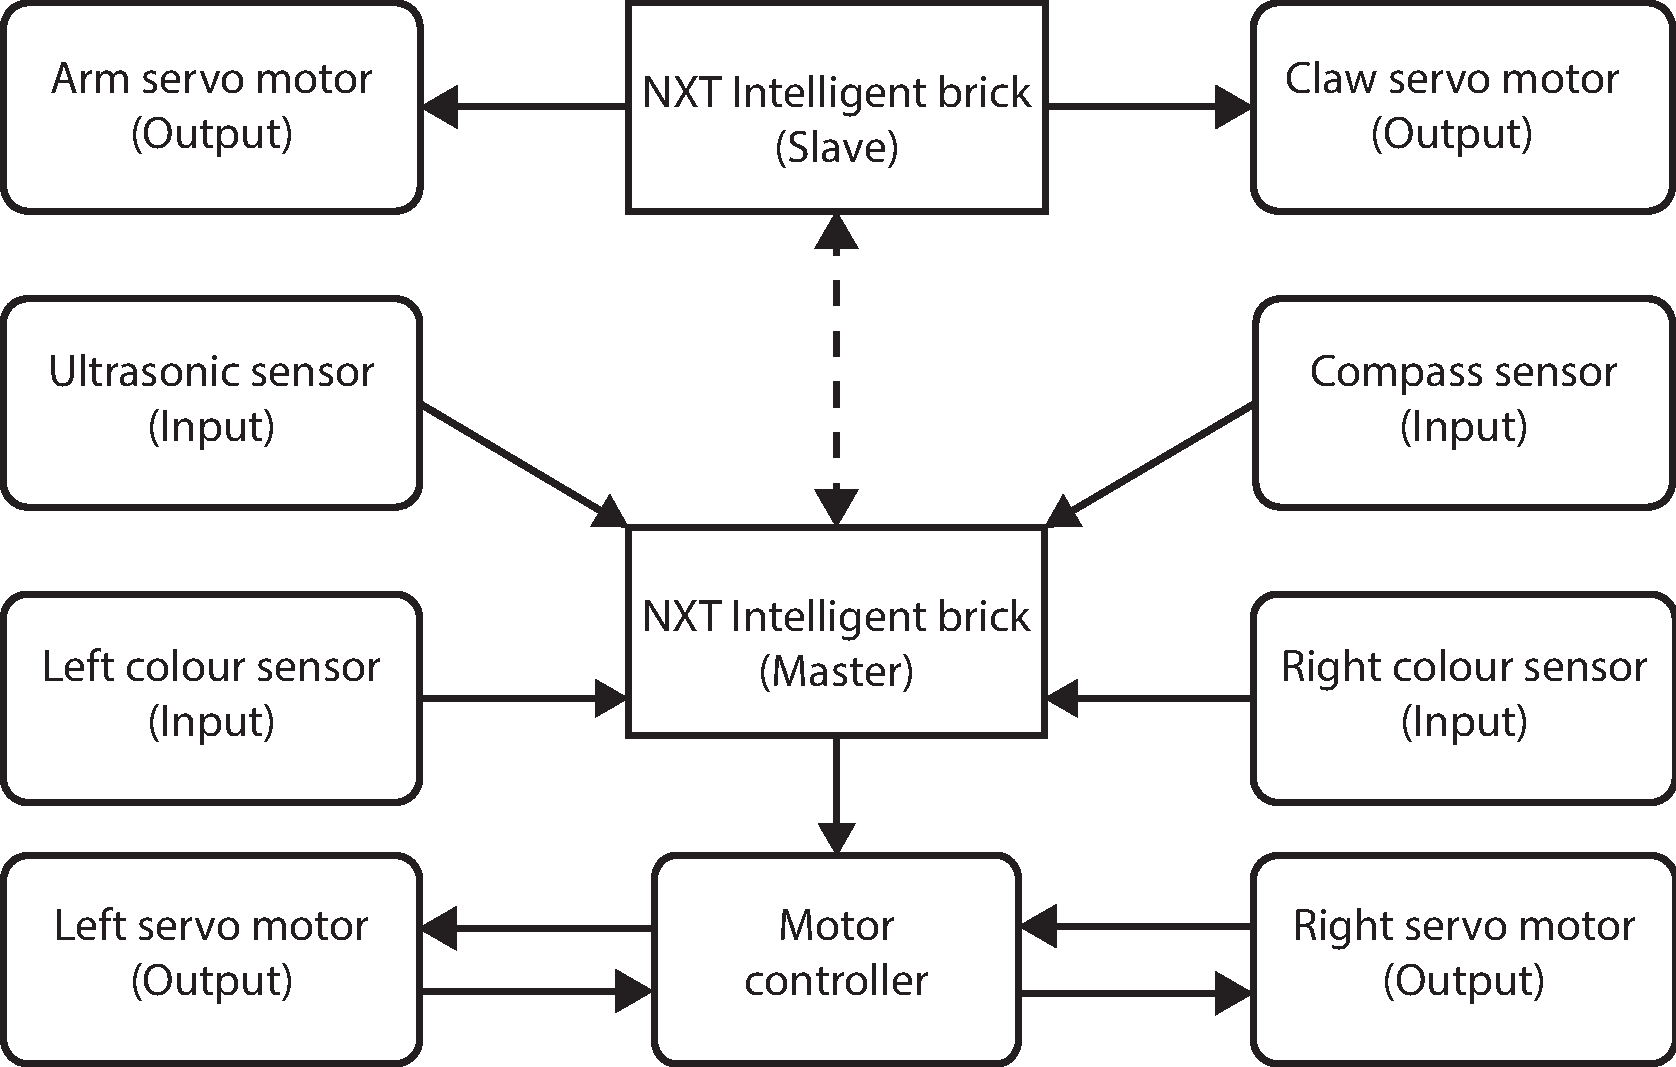
\includegraphics[width=\textwidth]
     {graphics/ComponentDiagram.pdf}}
     \caption{\label{fig:robot_overview} Diagram of all the components included in the robot.}
\end{figure}



% Algorithm design
\section{Algorithm design} \label{sec:algorithm-design}

In order to solve the \emph{travelling salesman problem}, as described in \secref{sec:problem-description}, a heuristic is needed. Since it is not feasible to solve the problem of finding the optimal path, an algorithm that provides an acceptable solution will be chosen instead.

Two algorithms have been proposed and designed in this project: one is more intelligent and takes all the relative distances between the objects into account, while the other is very reactive. These two algorithms are, respectively, the \emph{nearest neighbour (NN) algorithm} and the \emph{next-in-view (NIV) algorithm}.


\subsection{Nearest neighbour algorithm} \label{sec:nn-algorithm}
The NN-algorithm starts by doing a 360 degrees turn while scanning the nearby area around it for objects. The distance and angle for each object are saved and when the robot is done scanning, a route will be calculated using trigonometry and the NN-algorithm concepts. These calculations will result in an array of instructions containing distances and angles. Each instruction will take the robot from the current position to the next object following the calculated route. The robot should scan after completing the route, to ensure that all objects has been collected, in case it didn't collect all of the objects. The \projname{} computes the entire route before moving.

The algorithm uses trigonometry to select the next object, by using the current position, the starting position and the position of the next object. These positions are in relation to the starting position, where all the objects positions were found. The amount of degrees the \projname{} must turn, in order to get to the same heading as the next object, is saved as instructions, along with the distance that needs to be travelled in order to get to it. 

These instructions must then be followed after the route has been calculated. \figref{fig:object_navigation_first} shows a situation where all the objects have been spotted, and now the \projname{} must decide which object that should be collected first. At this point the shortest object is easy to conclude, as the distance to all objects, from the starting position, is already known, based on information from the ultrasonic sensor. The shortest distance overall is found, and saved along with the heading, and the object associated to this is remembered, and marked as collected, to remove this from consideration when finding the next objects. Another set of instructions is used to ensure that the \projname{} is pointing back, at the starting position. This is used to ease the calculations of the following objects. 

\begin{figure}[H]
     \center{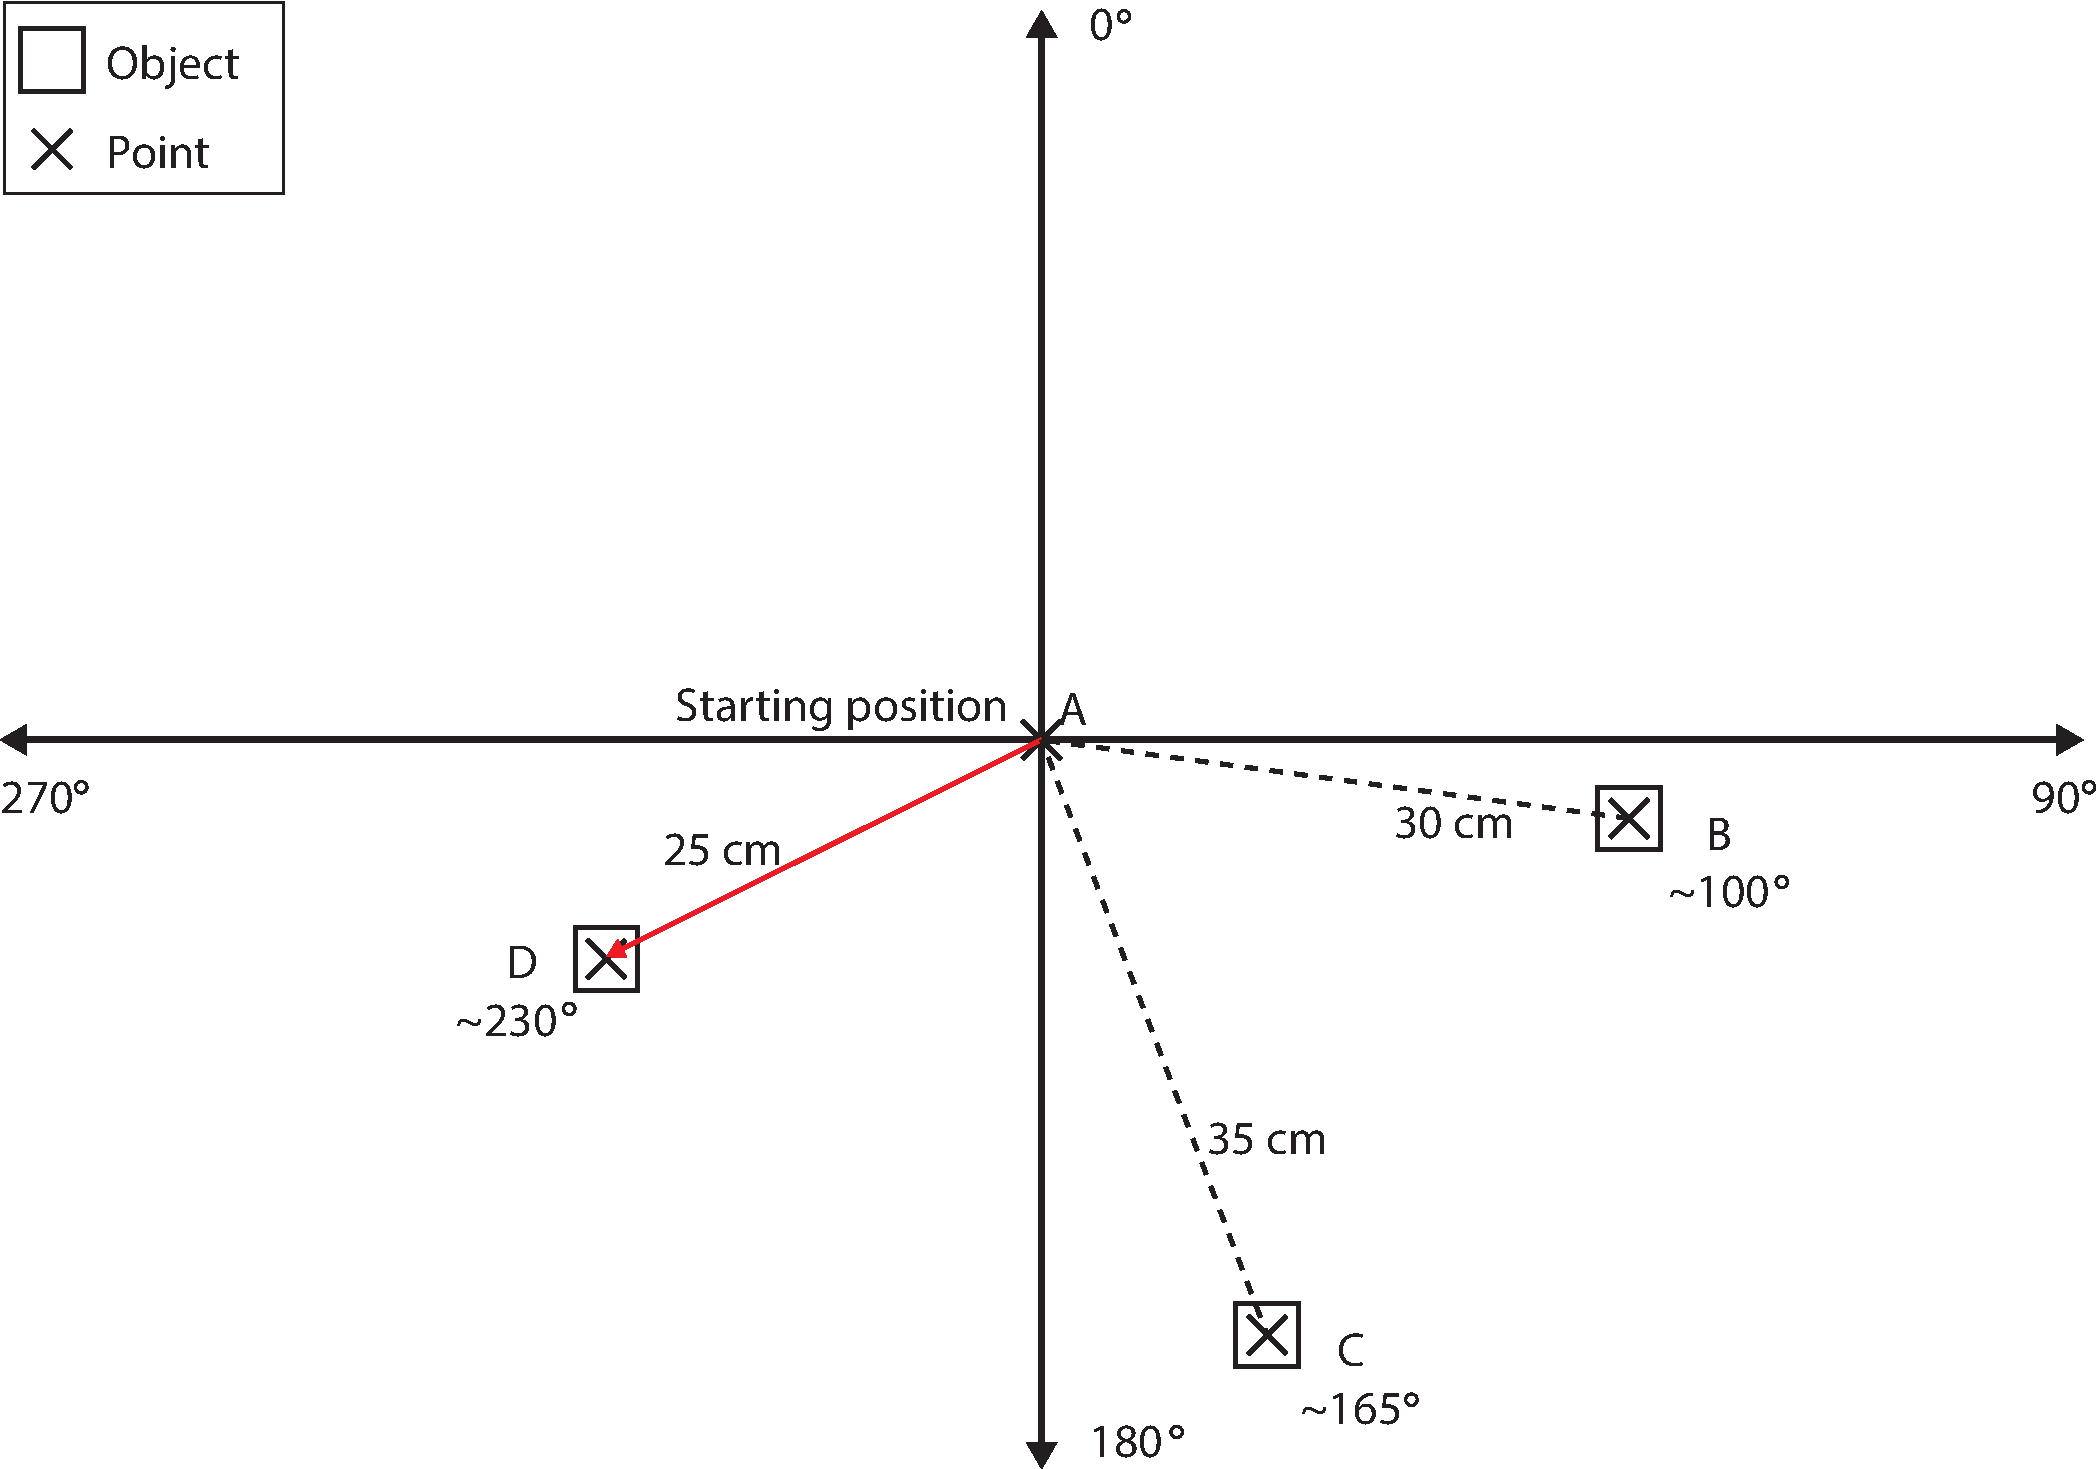
\includegraphics[width=\textwidth]
     {graphics/ObjectNavigationFirst.pdf}}
     \caption{\label{fig:object_navigation_first} First object to be collected.}
\end{figure}

Now that the first object has been scheduled to be collected, the NN-algorithm uses trigonometry to find the shortest distance to the next object, and calculates the angles that is needed to turn, to face the next object. The distance to all the other objects must be calculated, in order to find the closest one. To increase the understanding, the state of the world is represented in \figref{fig:object_navigation_iteration}, where the actions to collect the first object has been applied and reflected in the figure. From this point, the distance to the remaining objects is calculated, using the formula:
\begin{equation}
a = \sqrt{ b^2 + c^2 - 2*b*c*cos(A) } \label{equation:a}
\end{equation}

But for this, the A angle is needed. This is calculated from the spotted angles during the search. The formula for calculating A is:
\begin{equation}
A = (Object~currently~at~spotted~angle) - (Object~closest~spotted~angle) \label{equation:AAngle}
\end{equation}

With the same method as the first object, the object with the shortest distance, from the current object, is found and saves the object number. Now the heading to the closest object must be calculated, and this is the angle calculated by the formula:
\begin{equation}
B = cos^{-1}((a^2 + c^2 - b^2)/(2*a*c)) \label{equation:B}
\end{equation}

This provides the angle that must be turned in order to face the next object. In \figref{fig:object_navigation_iteration} the \projname{} is pointed towards the starting position, and the angle that must be turned is calculated from equation \ref{equation:B}. The current heading added/subtracted (depending on the position) with the angle provides the heading to the next object. This angle is added to the instructions along with the distance. Then the final angle of the triangle is calculated, which is used to turn the \projname{} towards the starting position again. The final angle is calculated with the formula:
\begin{equation}
C = 180 - A - B \label{equation:C}
\end{equation}

In order to point the \projname{} at the starting position again, the current heading is subtracted with (180 - C), where C is found by equation \ref{equation:C}. This process has provided the route to the next object, and the instructions to turn the \projname{} back, facing the starting position. The second step is executed for the remaining objects that were spotted. 

\begin{figure}[H]
     \center{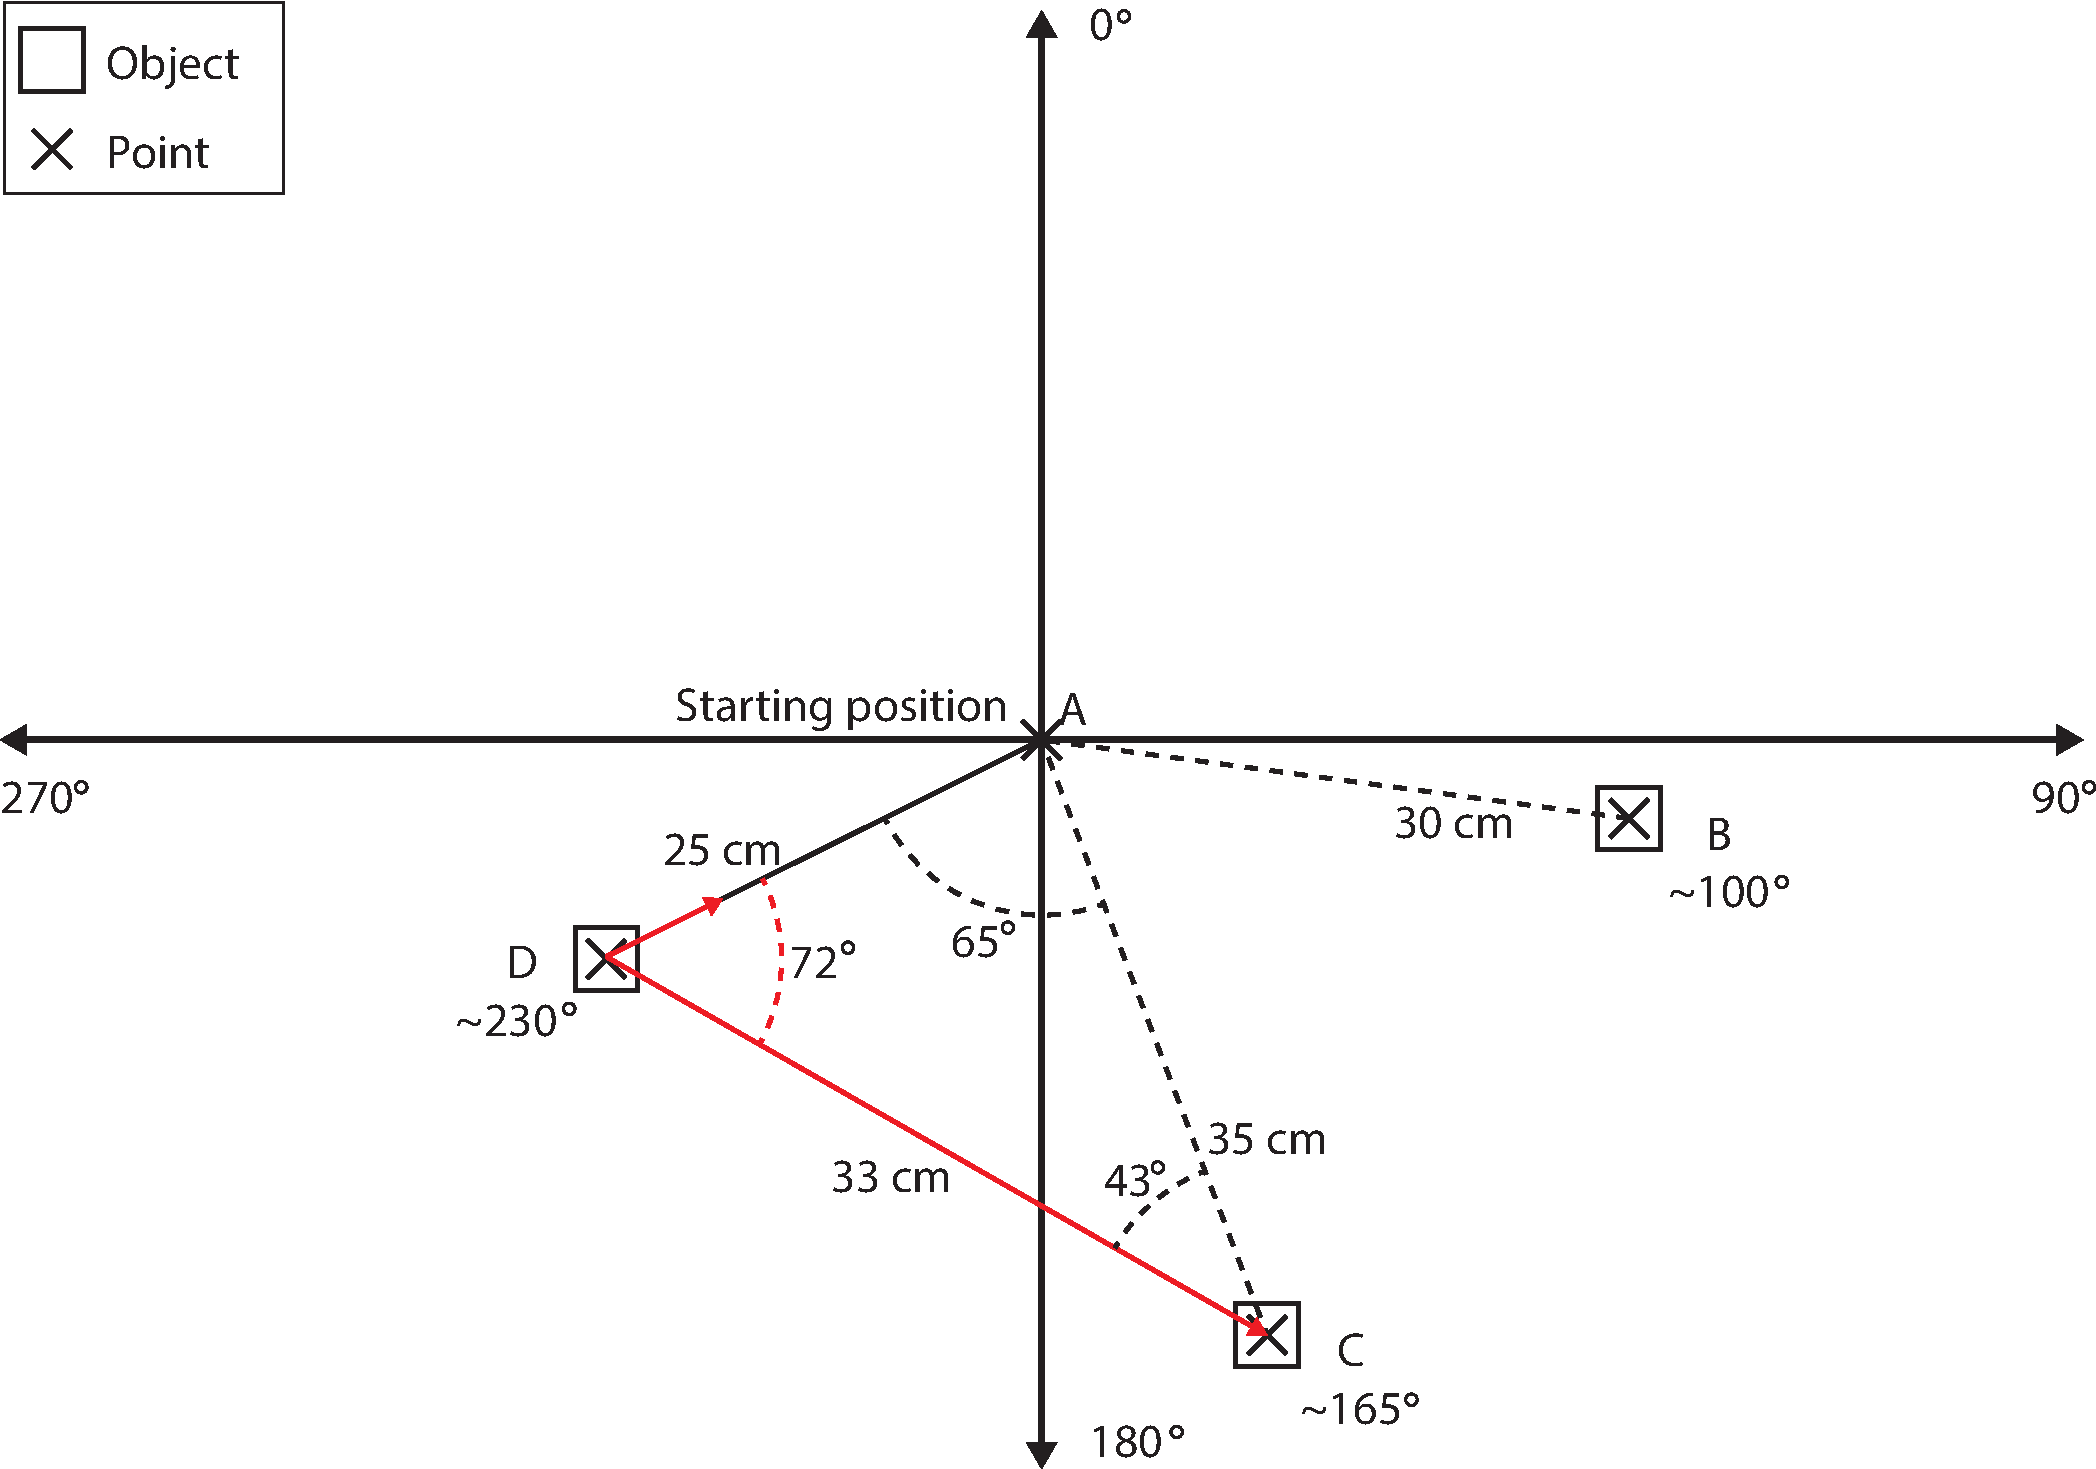
\includegraphics[width=\textwidth]
     {graphics/ObjectNavigationIteration.pdf}}
     \caption{\label{fig:object_navigation_iteration} Iteration of objects to be collected.}
\end{figure}


\subsection{Next-in-view algorithm} \label{sec:niv-algorithm}
An important property of the Next-in-view algorithm, is that it does not do any calculations prior to moving for objects, like the NN-algorithm. However it still relies a lot on the ultrasonic sensor, but in a different way. Instead of using the ultrasonic sensor to map the objects during the initial scan until all objects has been found, it uses the inputs from the sensor until all objects have been collected.

\begin{figure}[H]
     \center{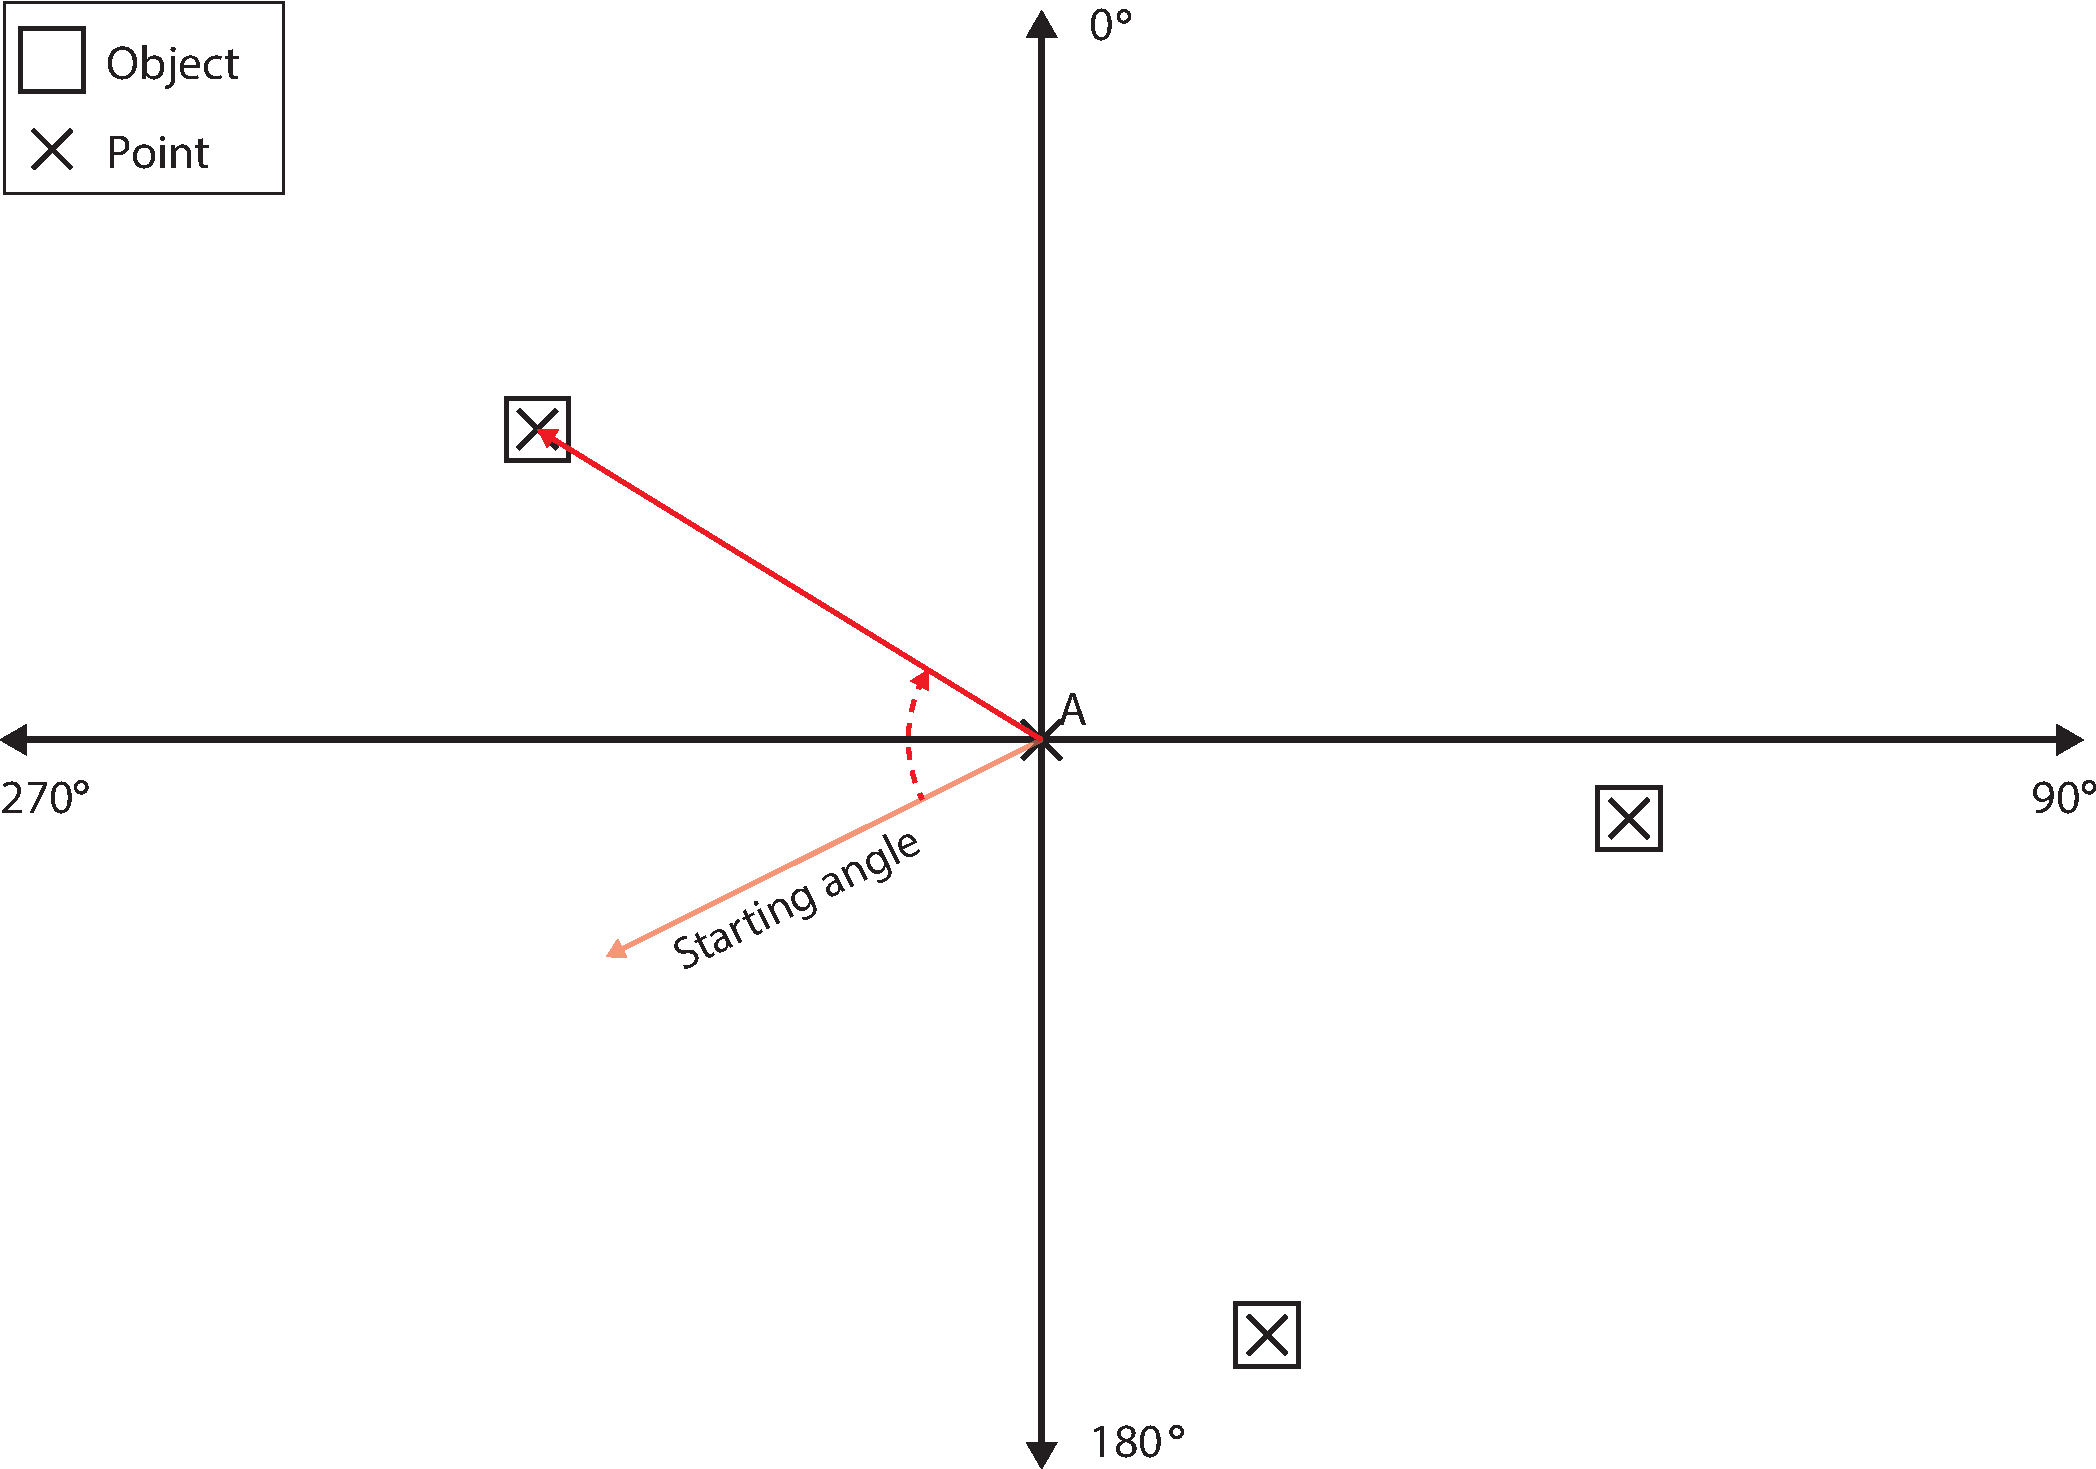
\includegraphics[width=\textwidth]
     {graphics/ObjectNavigationNIV.pdf}}
     \caption{\label{fig:object_navigation_niv} Start-up using the Next-in-view algorithm}
\end{figure}

At start-up the robot starts turning until it spots an object with the ultrasonic sensor, as seen in \figref{fig:object_navigation_niv}. It then drives towards it until the object is within grabbing distance of the claw. The object will be picked up and the \projname{} continues to search for objects, as seen in \figref{fig:object_navigation_niv2}

\begin{figure}[H]
     \center{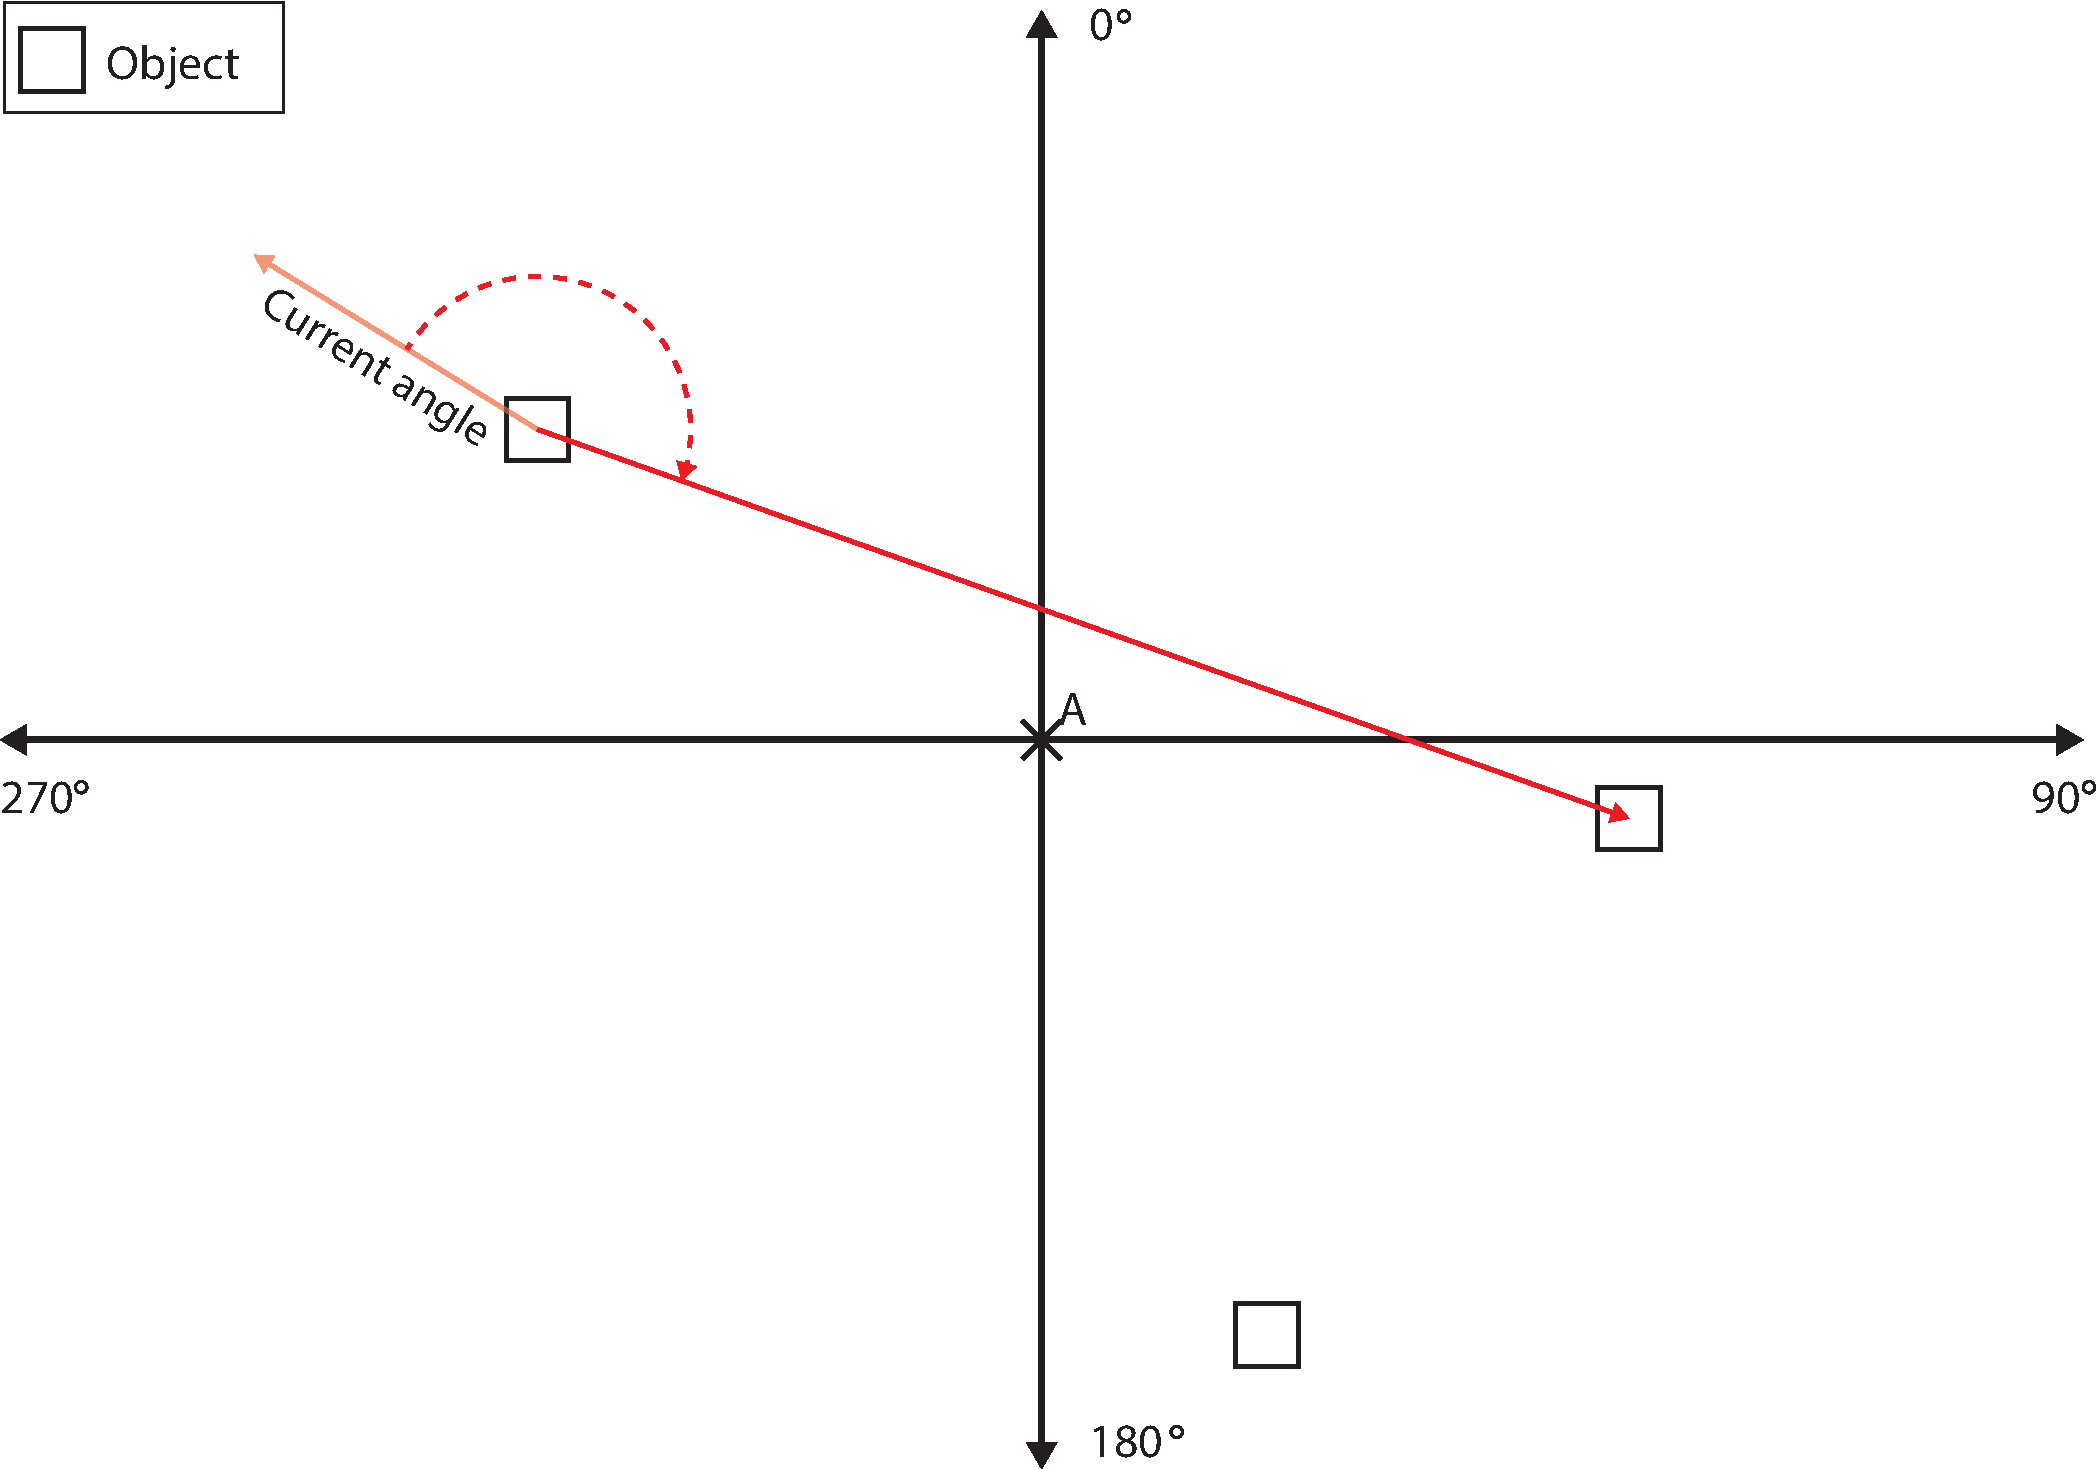
\includegraphics[width=\textwidth]
     {graphics/ObjectNavigationNIV2.pdf}}
     \caption{\label{fig:object_navigation_niv2} Searching for the next object}
\end{figure} 

Because the ultrasonic sensors view is a cone, as described in \secref{sec:hardware}, a case may arise where the robot is not driving straight towards the object. And as it gets closer, it might lose the object as it gets out of the view of the sensor.

In this case, a small routine will be initiated, where the robot will turn a little to the right, followed by a little to the left, constantly scanning for objects, while slowly increasing the angles turned to scan an increasingly larger range. When an object is spotted again, the robot continues to move towards it. When the object has been collected, the robot starts turning until it finds a new object and the entire process continues until every object has been found.


\subsection{Algorithm comparison} \label{sec:algorithm-desc}

The shortest route between the objects can be brute forced by trying out every single possible route between the start position and all of the objects. This would have a calculation time of $\mathcal{O}(n!)$, which means that with every object added, the running time greatly increases. This gives the robot problems when calculating the shortest route, if the amount of objects exceeds a certain number, due to its limited processing power. If there are 9 objects for instance, the number of different paths to check exceeds 360,000.  

A faster, but less distance-efficient algorithm is the NN-algorithm. The algorithm calculates a route based on which objects are closest together. This means that the distance to all the points are calculated from the starting point and the shortest distance is chosen. This is then repeated from the new point, but this time it does not include the objects from previously visited points. This results in a worst case calculation time of $\mathcal{O}(n^2)$, although as the number of remaining objects decreases for each object added to the route, described by $\sum\limits_{i=n}^n i = i - 1$, the calculation time decreases for each object. Compared to the brute force, this algorithm uses only a fraction of the time to compute the result. 

An algorithm that doesn't spend time on calculations prior to moving for objects is the next-in-view algorithm. This algorithm has a number of issues connected to it, which may reduce its performance, however in smaller cases with less than ten objects, its completion speed is close to the NN-algorithm. This is based purely on a theoretical test calculation.

\begin{figure}[H]
     \center{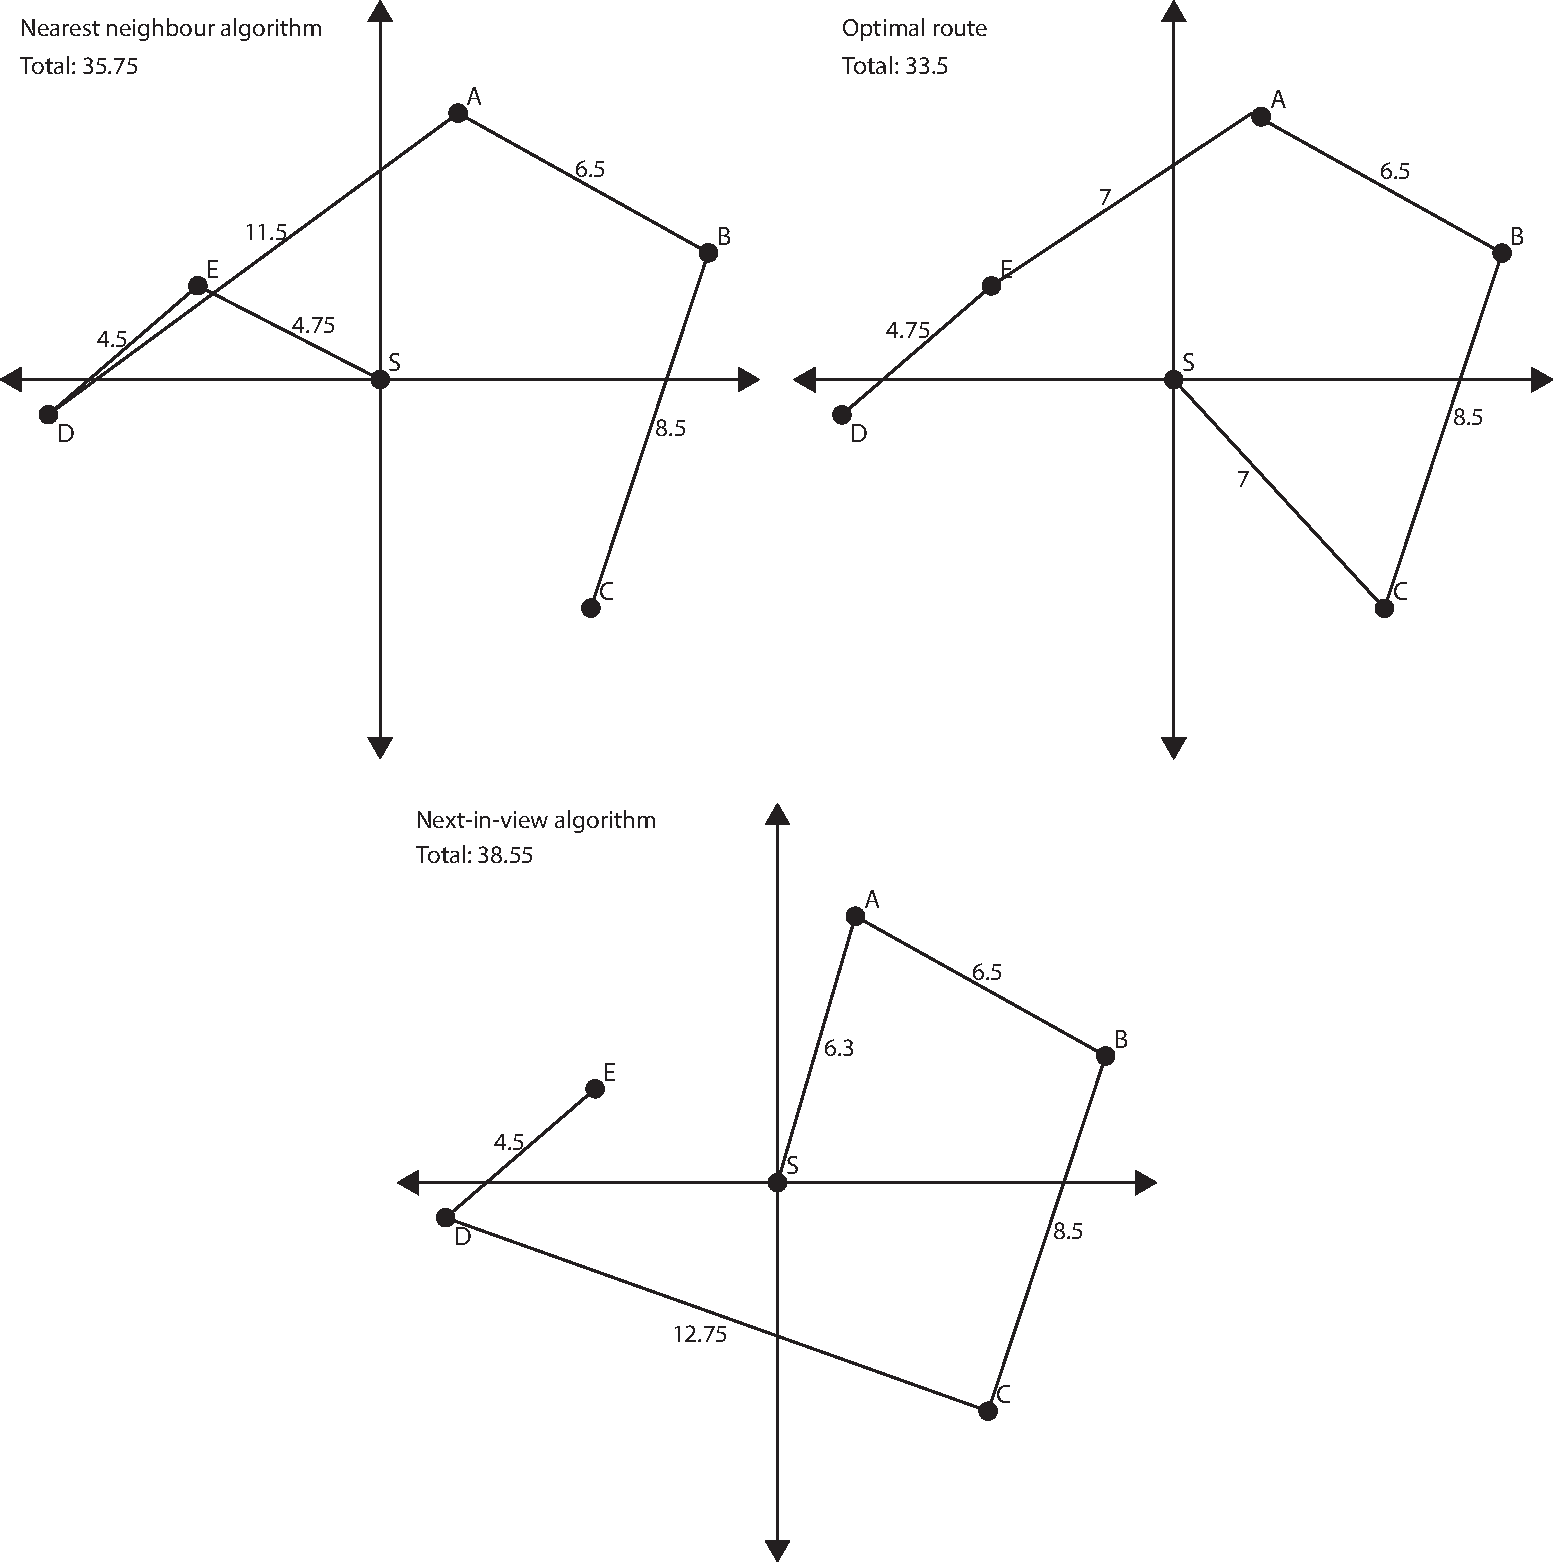
\includegraphics[width=\textwidth]
     {graphics/AlgorithmExamples2.pdf}}
     \caption{\label{fig:algorithm-example} Example of the NN-algorithm, the optimal solution, and next-in-view algorithm.}
\end{figure}

\figref{fig:algorithm-example} shows three solutions to the problem. The top right graph is the optimal solution, which is only used to compare the results from the two other algorithms. Top left is the NN-algorithm, and in the bottom the next-in-view algorithm. The robot starts its route at position \emph{S}. The objects are named in order as they are first detected, if scanning clockwise. The algorithms result in the routes shown on the figure.

The different algorithms result in the routes shown in \figref{fig:algorithm-example}, and have following lengths:
\begin{itemize}
\item Optimal: 33.5 units
\item Nearest neighbour algorithm: 35.75 units
\item Next-in-view: 38.55 units
\end{itemize}

In the average case, the difference between the NN-algorithm and the NIV solutions would be larger if there were more objects to consider. However for these smaller cases, the difference is almost negligible. It should be noted, that this does not describe the time spent, only the distance travelled: rotation to scan for objects, for both algorithms, takes different amounts of time depending on the case. This is not accounted for here.

Due to the limitations of the LEGO NXT brick and the complexity of the problem, finding the optimal solution was ruled out as a possibility. The NN-algorithm maps all objects in the environment, and constructs a route to all the objects before it begins collecting them. The NIV-algorithm is very ad hoc in nature, in that it simply goes for the first object that the robot spots after each scanning cycle is initiated. 

The NN-algorithm is expected to yield the most efficient results, however based on the hardware test of the ultrasonic sensor in \secref{sec:ultrasonic_sensor}, it was deemed unlikely that it would work in practice, since it heavily relies on accurate information about the location of objects in the environment. Due to this, the NN-algorithm was designed in the case that it would work in practice, however the NIV-algorithm was designed and implemented first, as insurance that the robot would be able to complete its task, however not as efficiently.

As mentioned in the test case from \secref{sec:nn-algorithm}, the difference between the two algorithms' distance were nearly insignificant. This also means that using a state-based representation of the world is preferred, where each state represents the robots behaviour. If the NN-algorithm were used, a feature based representation would be better suited for the \projname{}, because of the need to map the location of each found object in relation to the environment.



% Requirement specification
\section{Requirement specification} \label{sec:requirement_specification}

The final version of \projname{} is an autonomous robot that is able to navigate within a marked environment. Within this environment it is able to locate and collect various objects and store them.

\subsection{Requirements}

\projname{} has the following physical features:

\begin{itemize}
    \item \textbf{Tank treads}\\
        Instead of wheels, the \projname{} is equipped with tank treads. This allows the robot to turn around its own axis while not moving away from the position. The tank treads provides the \projname{} with a better grip on a multitude of surfaces.
    \item \textbf{Robotic arm to collect objects}\\
        Consisting of 2 servo motors, this arm has two moveable joints: one to move the arm itself from the front of the \projname{} where it is mounted to the back, and one to control the claw that grabs hold of objects.
    \item \textbf{Sensors to detect objects, environment boundaries and the heading of the robot}\\
        Two colour sensors, one in each front corner. Between those sits an ultrasonic sensor to detect distance. A compass sensor is stably mounted 10 cm above the NXT bricks and at least 15 cm from the motors to avoid any magnetic disturbance.
    \end{itemize}
    
The \projname{} is able to perform the following actions:

    \begin{itemize}
    \item \textbf{Navigate the environment within the boundaries}\\
        The robot is able to move around within the environment, as described in \secref{sec:delimitation}, while searching for objects to collect. If it encounters a boundary, it is able to navigate itself back and find a new direction.
    \item \textbf{Control collection arm to pick up and store objects of specified size}\\
        When an object is detected in the correct position, the \projname{} is able to pick it up and store it, using its motorised arm and claw.
    \item \textbf{Find and collect all objects within reasonable time}\\
        The \projname{} is able to find, collect and store all objects within the environment within the time limit set in \secref{sec:model}.
\end{itemize}





%\subsection{Testing}
%The robot and its functions were tested in various different stages. As in the implementation procedure, the functions were tested individually. The individual functions were then combined one by one while being tested simultaneously, until the robot was fully assembled. The first round of tests can be seen in \secref{sec:hardware} while the final overall test can be found in \charef{cha:quality-assurance}. 

%The final version of \projname{} will consist of a set of tank treads for movement and navigation, a movable arm with a functional claw for grabbing objects, a colour sensor to detect the border of the environment, and a storage container on the back for storing the collected objects. The robot's LEGO components and their functionality can be found in \secref{sec:functionality_description}. The robot will be able to navigate within the environments boundaries and find objects which it will collect and store in its container.
